\documentclass[10pt]{standalone}
\usepackage{tikz}
\usepackage{pgfplots}
\usepackage{filecontents}
\usepackage{amsmath}

\begin{document}

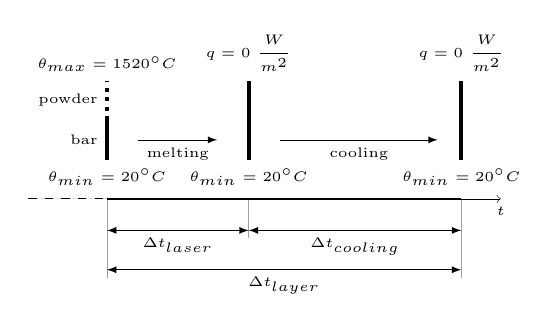
\begin{tikzpicture}
    [ timebar/.style={black,draw=black, fill=black, fill opacity=1},
      bar/.style={black,draw=black, fill=black, fill opacity=1, line width=0.5mm},
      dashedBar/.style={black,draw=black, fill=black, fill opacity=1, dashed},
      grid/.style={very thin, black, draw=gray!75},
      axis/.style={black,<->,>=latex, very thin},
      arrow/.style={black,->,>=latex, very thin},
      arrowTime/.style={black,->, very thin},
      load/.style={black,fill=gray!70, fill opacity=0.4},
      dim/.style={latex-latex}]
      
  \scriptsize%



%%%%%%%%%%%%%%%%%%%%%%%%%%%%%%%%%%%%%%%%%%%%%%%%%%%%%%%%%%%%%%%%%%%%%%%%%%%%%%%%%%%%%%%%%%%%%%%%%%%%%%%%%%
%draw layer time discretization
	  % draw element
	  scale = 2.0;
	  \draw[timebar]   (0.0,0.0,0.0) -- (+2.25 * 2,0.0,0.0);
	  \draw[dashedBar]   (-0.5*2,0.0,0.0) -- (0.,0.0,0.0);
	  
	  \draw[grid] (0.0,0.0,0.0) -- (0.0,-0.5*2,0.0);	  
	  \draw[grid] (0.9*2,0.0,0.0) -- (0.9*2,-0.25*2,0.0);	  
	  \draw[grid] (2.25*2,0.0,0.0) -- (2.25*2,-0.5*2,0.0);	 
	  
	  \draw[axis] (0.0,-0.2*2,0.0) -- (0.9*2,-0.2*2,0.0) node[ midway, below] {\tiny $\Delta t_{laser}$};
	  \draw[axis] (0.9*2,-0.2*2,0.0) -- (2.25*2,-0.2*2,0.0) node[ midway, below] {\tiny $\Delta t_{cooling}$};
	  \draw[axis] (0.0,-0.45*2,0.0) -- (2.25*2,-0.45*2,0.0) node[ midway, below] {\tiny $\Delta t_{layer}$};	
	  
	  \draw[arrowTime] (0.0, 0.0, 0.0) -- (2.5*2, 0.0, 0.0) node[left, below] {\tiny $t$ };
  

%%%%%%%%%%%%%%%%%%%%%%%%%%%%%%%%%%%%%%%%%%%%%%%%%%%%%%%%%%%%%%%%%%%%%%%%%%%%%%%%%%%%%%%%%%%%%%%%%%%%%%%%%%
%insert bar evolution pics

	  \draw[bar]   (0.0, 0.5, 0.0) node[below] {\tiny $\theta_{min} = 20^{\circ}C$} -- (0.0, 1.0, 0.0)  node[left, midway] {\tiny bar};
	  \draw[black, dotted, line width=0.5mm](0.0, 1.0, 0.0)  -- node[left, midway]{\tiny powder}(0.0, 1.5, 0.0) node[above] {\tiny $\theta_{max} = 1520^{\circ}C$}; 
	  \draw[arrow] (0.2*2, 0.75, 0.0) -- (0.7*2, 0.75, 0.0) node[midway, below] {\tiny melting};
	  \draw[bar]   (0.9*2, 0.5, 0.0) node[below] {\tiny $\theta_{min} = 20^{\circ}C$} -- (0.9*2, 1.5, 0.0)node[above] {\tiny $q = 0$ $\dfrac{W}{m^{2}}$}; 
	  \draw[arrow] (1.1*2, 0.75, 0.0) -- (2.1*2, 0.75, 0.0) node[midway, below] {\tiny {cooling} };
	  \draw[bar]   (2.25*2, 0.5, 0.0) node[below] {\tiny $\theta_{min} = 20^{\circ}C$} -- (2.25*2, 1.5, 0.0)node[above] {\tiny $q = 0$ $\dfrac{W}{m^{2}}$}; 
  
\end{tikzpicture}
\end{document}